\section{System}
This section discusses the detail of our offline system. 
The goal of this part is to generate an Action-Noun mapping
from which we can obtain the noun abstraction of the 
action triple.
\subsection{Baseline method}
We take an intuitive approach as our baseline, which we call the most frequent noun.act. Given an action concept \emph{subject verb object} where \emph{subject} and \emph{object} are both concept, e.g., country invade country. $S_{verb}$ is the set of verb's synonyms in WordNet. Since an action triple doesn't provide adequate information for verb sense disambiguation, we take all synsets as verb's synonyms. $D_{verb}$ is the the set of all derivationally related words of verbs in $S_{verb}$, from which we choose those whose semantic field (lexical file name) in WordNet is noun.act. The first-K nouns with highest total frequency counts are taken as our candidates.
\begin{equation*}
    S_{verb} = \{{ v \in S_i | S_i \ synset \ of \ verb}\}
\end{equation*}
\begin{equation*}
    D_{verb} = \{{ D_i \ d.r.w.  \ of \ s_i | s_i \in S_{verb}}\}
\end{equation*}


\figref{fig:baseline} shows how it works.


\begin{figure}[h]
\includegraphics[width=\columnwidth]{img/baseline.eps}
\caption{Baseline method}
\label{fig:baseline}
\end{figure}

\subsection{Retrieval based method}

Under the assumption that nouns in news titles are likely to be good candidates
for abstraction of action instances in the news bodies, we use a TF-IDF based retrieval method
to find the action-noun mapping.

We first build our noun dictionary $D$. Here the main sources we use are Wordnet, 
Probase and Wikitionary.
\begin{figure}[h]
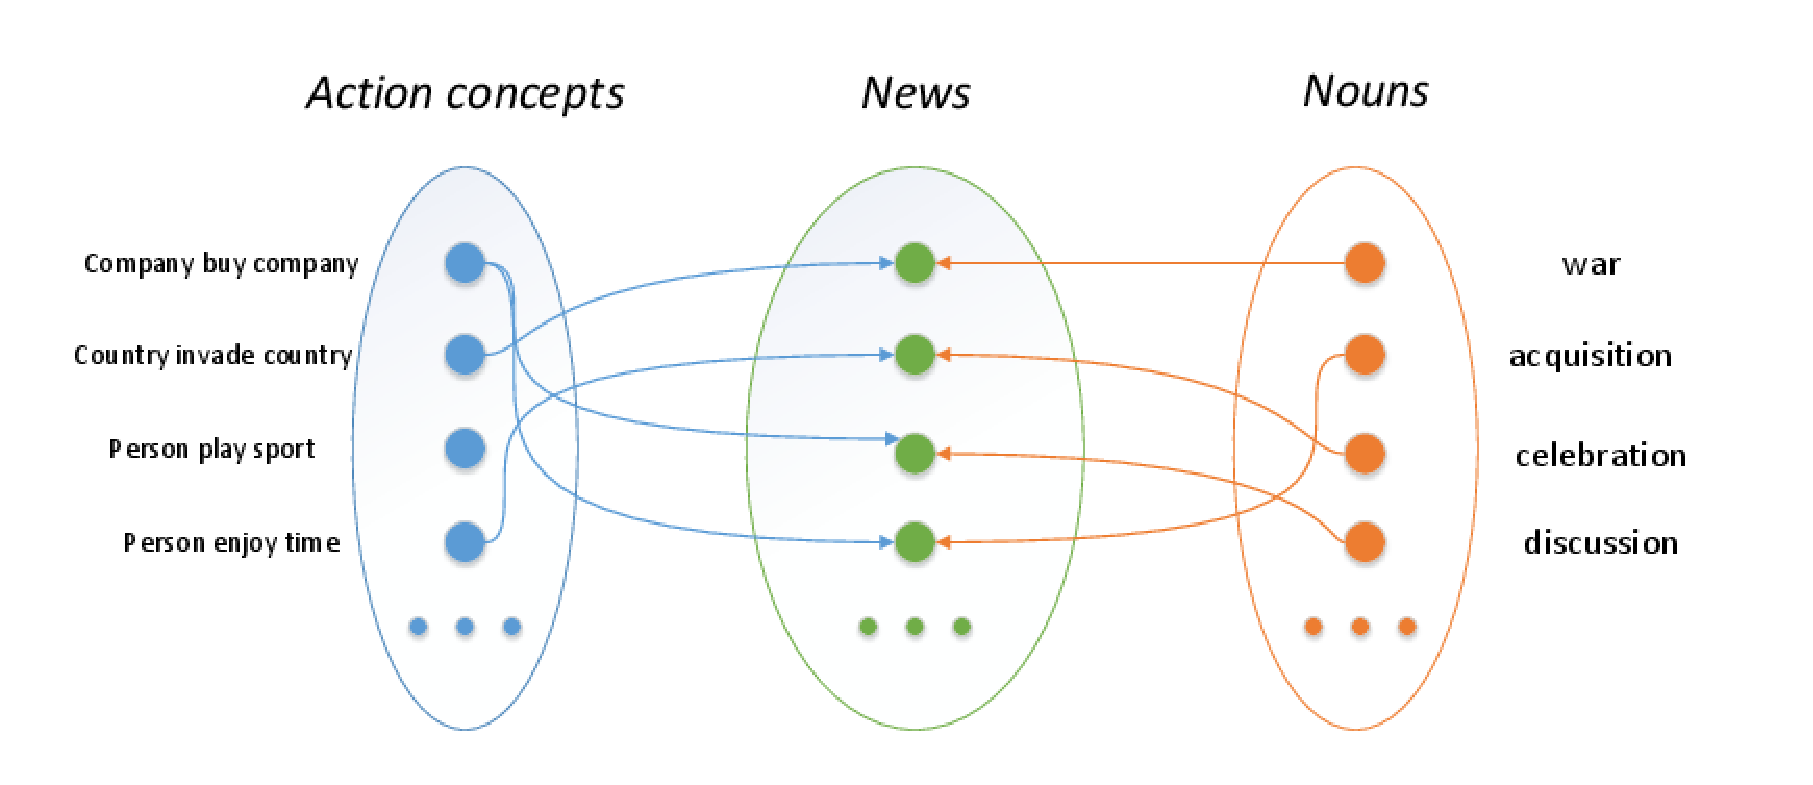
\includegraphics[width=\columnwidth]{img/ac2}
\caption{Tripartite Graph}
\label{fig:tripartite}
\end{figure}


Next we find the distribution of noun concepts in news titles, $f_n(i)$, and the distribution of action instances in news bodies, denoted as $f_{ac}(i)$ 
\begin{align*}
    f_n(i) & = \{ j |  i \in t_j \} \\
    f_{ac}(i) &= \{ k | i \in b_k \}
\end{align*}
where $t_i$ and $b_i$ are title and body of $i^{th}$ news, respectively. 

Next we use TFIDF to compute the relatedness of nouns to actions. 
\begin{equation*}
    freq(n_i, ac_j) = \bigm| \{ k | n_i \in t_k \land ac_j \in b_k \} \bigm|
\end{equation*}
\begin{eqnarray*}
&& TF(n_i, ac_j) = \\
&&\begin{cases} 0 &\mbox{if freq is 0} \\
        1 + \log(freq(n_i, ac_j)) &\mbox{otherwise}
    \end{cases}
\end{eqnarray*}


\begin{equation*}
    docfreq(n_i) = \bigm|\{ k | n_i \in t_k \}\bigm|
\end{equation*}


\begin{equation*}
    IDF(n_i) = log(\frac{\text{news corpus size}}{1 + docfreq(n_i)})
\end{equation*}

\subsection{Search Engine}
After obtaining the Action-noun mapping, we are ready to construct the search engine
with conditional semantic search. Here we use around 39000 BBC news as our dataset.
In order to extract the webpages with action instances, we need to traverse the 
news dataset offline. Specifically, we find each occurrence of action instances
in the dataset, and with our Action-noun mapping we could obtain multiple noun abstractions
for these instances. Then we add these news to the index of those nouns, to achieve the
effect that as if those nouns are mentioned in the original news.

If the query itself is an action concept or action instance, we need to convert it into 
several noun concepts and expand the query. After some preliminary experiments we decide
to expand action concept as the verb OR noun concept, for example if the query is ``country
invade country'', the query will be converted to ``invade OR war''. If the query is an 
action instance, for example ``Google buy company'', we will keep the argument instance
. So in this example it will be converted to ``Google AND ( buy OR acquisition )''


\begin{figure}[h]
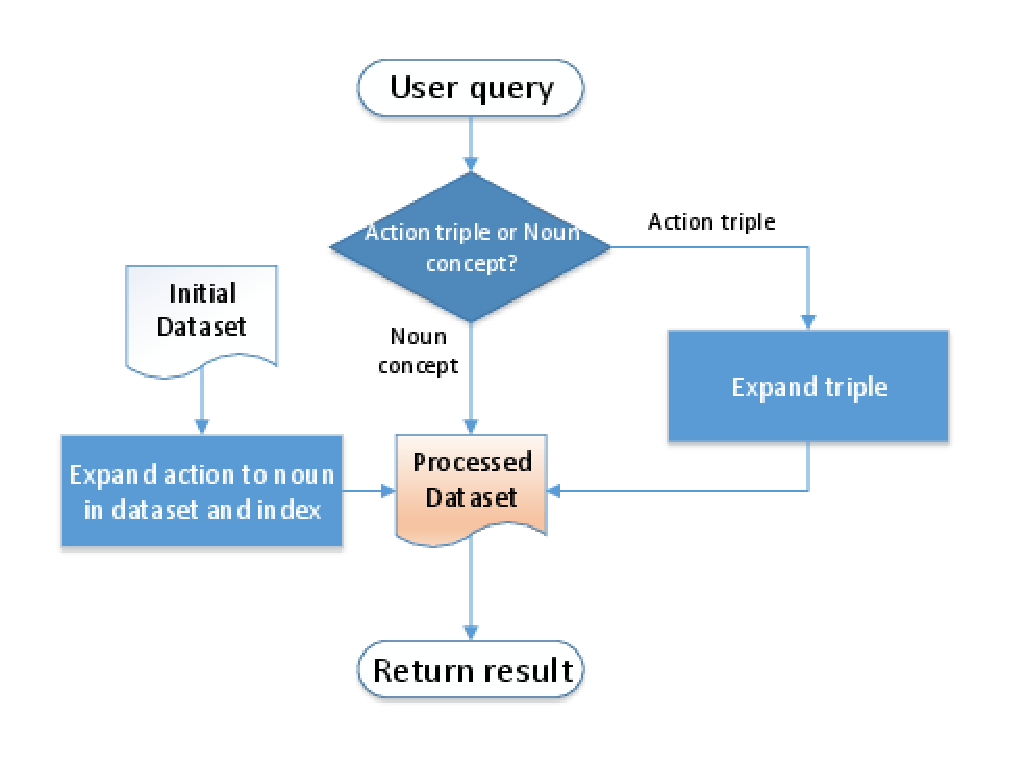
\includegraphics[width=\columnwidth]{img/ac4}
\caption{Search engine workflow}
\label{fig:search engine}
\end{figure}


